\section{导数}\label{zhang_derivative}
\subsection{定义}
导数的概念从物理发展出来的。
$$v\left(t_0\right)=\lim\limits_{\vartriangle t\to 0}\frac{s\left(t_0+\vartriangle t\right)-s\left(t_0\right)}{\vartriangle t}$$
\begin{figure}[htp]
  \centering
  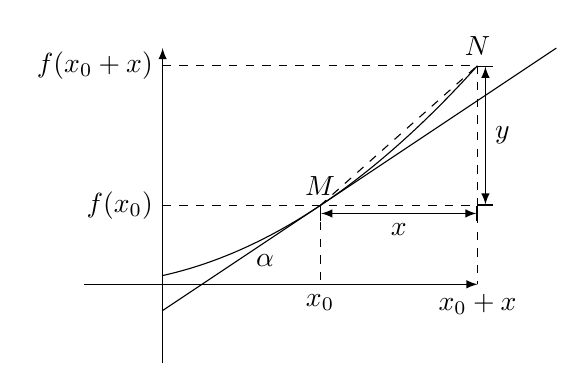
\begin{tikzpicture}[>=latex]
    \draw[->](0,0)--(5,0);
    \draw[->](1,-1)--(1,3);
    \draw[domain=1:5,samples=1000] plot(\x,{(\x^2)/9});
    \draw[domain=-2:3,samples=1000] plot(\x+3,{\x*(2/3)+1});
    \draw[dashed] (3,{(3^2)/9})--(3,0)node[below]{$x_0$};
    \draw[dashed] (3,{(3^2)/9})node[above]{$M$}--(5,{(5^2)/9})node[above]{$N$};
    \draw[dashed] (5,{(5^2)/9})--(5,0)node[below]{$x_0+\vartriangle x$};
    \node at (2.3,.5)[below]{$\measuredangle \alpha$};
    \draw[dashed] (1,{(3^2)/9})node[left]{$f(x_0)$}--(3,{(3^2)/9})--(5,{(3^2)/9});
    \draw[|<->|] (3,{(3^2)/9-.1})--(4,{(3^2)/9-.1})node[below]{$\vartriangle x$}--(5,{(3^2)/9-.1});
    \draw[dashed] (1,{(5^2)/9})node[left]{$f(x_0+\vartriangle x)$}--(5,{(5^2)/9});
    \draw[|<->|] (5.1,{(3^2)/9})--(5.1,{((5^2/9)+(3^2/9))/2})node[right]{$\vartriangle y$}--(5.1,{(5^2)/9});
\end{tikzpicture}
\end{figure}
$$NM\mbox{斜率}=\tan \beta=\frac{f\left(x_0+\vartriangle x\right)-f(x_0)}{\vartriangle x}=\frac{\vartriangle y}{\vartriangle x}$$
$$\mbox{斜率}k=\tan \alpha=\lim\limits_{\vartriangle x\to 0}\tan \beta=\lim\limits_{\vartriangle x\to 0}\frac{\vartriangle y}{\vartriangle x}=\frac{f\left(x_0+\vartriangle x\right)-f(x_0)}{\vartriangle x}$$
\subsubsection{导数定义}
$y=f(x)$在$x_0$的某邻域内有定义\\
给自变量的增量$\vartriangle x,\left(x_0+\vartriangle x\right)$仍在定义域内\\
函数得到了相应增量$\vartriangle y ,\vartriangle y =f\left(x_0+\vartriangle x\right)$\\
如果$\lim\limits_{\vartriangle x\to 0}\frac{f\left(x_0+\vartriangle x\right)-f(x_0)}{\vartriangle x}$存在,称$y=f(x)$在$x=x_0$处可导 \\
$\left(\mbox{极限值为}y=f(x)\mbox{在}x=x_0\mbox{处导数}\right)$
\begin{center}
  记$y'|_{x=x_0}=f'(x_0)=\lim\limits_{\vartriangle x\to 0}\frac{f(x_0+\vartriangle x)-f(x_0)}{\vartriangle x}=\lim\limits_{\vartriangle x\to 0}\frac{\vartriangle y}{\vartriangle x}$
  $$\lim\limits_{\vartriangle x\to 0}\frac{f(x_0+\vartriangle x)-f(x_0)}{\vartriangle x}\Leftrightarrow\lim\limits_{\vartriangle x\to x_0}\frac{f(x)-f(x_0)}{x-x_0}$$
\end{center}
\subsubsection{导函数定义}
$f(x)$在区间$I$内任意一点均可导。\\
$f'(x)=\lim\limits_{\vartriangle x\to 0}\frac{f(x_0+\vartriangle x)-f(x_0)}{\vartriangle x}$\\
称$f'(x)$为$y=f(x)$在区间$I$上的导函数
\subsubsection{闭区间可导定义}
$f(x)$在$[a,b]$可导$\Leftrightarrow\begin{cases}
  f'(x_0)  &x_0\in(a,b)\Leftrightarrow\begin{cases}
    \mbox{左导数}f_-'(x_0)=\lim\limits_{\vartriangle x\to 0^-}\frac{f(x_0+\vartriangle x)-f(x_0)}{\vartriangle x}\\
    \mbox{右导数}f_+'(x_0)=\lim\limits_{\vartriangle x\to 0^+}\frac{f(x_0+\vartriangle x)-f(x_0)}{\vartriangle x}
  \end{cases}\\
  f_+'(a) &x=a\\
  f_-'(a) &x=b
\end{cases}$
\subsubsection{导数与连续}
\begin{align}\label{derivative_continuity}
  f'(x)\mbox{存在}\Rightarrow f(x)\mbox{在}x=x_0\mbox{处连续}
\end{align}
\subsection{幂数,指数,对数}
\begin{align}
&(C)' = 0\label{derivative_1} \\
&(x^a)' = ax^{a-1} \label{derivative_2} \\
&(a^x)' = a^x\ln a \label{derivative_3}\\
&(e^x)' = e^x \label{derivative_4}\\
&(\log_a^x)' = \frac{1}{x\ln a} \label{derivative_5}\\
&(\ln{x})' = \frac{1}{x} \label{derivative_6}
\end{align}
\subsection{三角函数}
\vspace{-10mm}
\begin{align}
&(\sin x)' = \cos x \label{derivative_sin}\\
&(\arcsin x)' = \frac{1}{\sqrt{1-x^2}} \label{derivative_arcsin}\\
&(\csc x)' = -\csc x\cot x \label{derivative_csc}\\
&(\cos x)' = -\sin x \label{derivative_cos}\\
&(\arccos x)' = -\frac{1}{\sqrt{1-x^2}} \label{derivative_arccos}\\
&(\sec x)' = \sec x\tan x \label{derivative_sec}\\
&(\operatorname{arcsec}{x})'=\frac{1}{\left|x\right|\sqrt{x^2-1}} \label{derivative_arcsec}\\
&(\tan x)' = \sec^2x \label{derivative_tan}\\
&(\arctan x)' = \frac{1}{1+x^2} \label{derivative_arctan}\\
&(\cot x)' = -\csc^2x \label{derivative_cot}\\
&(\operatorname{arccot}{x})' = -\frac{1}{1+x^2}\label{derivative_arccot}\\
&(\sinh x)' = \cosh x \label{derivative_sinh}\\
&(\cosh x)' = \sinh x \label{derivative_cosh}\\
&(\tanh x)' = \frac{1}{cosh^2 x}=1-\tanh^2x \label{derivative_tanh}\\
&(\operatorname{arcsinh}{x})' =\frac{1}{\sqrt{x^2+1}} \label{derivative_arcsinh}\\
&(\operatorname{arccosh}{x})'=\frac{1}{\sqrt{x^2-1}} \label{derivative_arccosh}\\
&(\operatorname{arctanh}{x})'=\frac{1}{1-x^2} \label{derivative_arctanh}
\end{align}
\subsection{导数运算}
\begin{center}
  \text{ $u=u(x),v=v(x),\mbox{均在}x\mbox{点可导},C\mbox{为常数}$}
\end{center}
\begin{align}
  (Cu(x))'&= Cu'(x)\label{limit_operation_1}\\
  (u(x)\pm v(x))'&=u'(x)\pm v'(x)\label{limit_operation_2}\\
  (u(x)\cdotp v(x))'&=u'(x)v(x)+v'(x)u(x)\label{limit_operation_3}\\
  \left(\frac{u(x)}{v(x)}\right)'&=\frac{u'(x)v(x)-v'(x)u(x)}{\left[v(x)\right]^2}\label{limit_operation_4}
\end{align}
\subsection{反函数求导}
如果函数$y=f(x)$在区间$(a,b)$内单调可导,且$f'(y)\neq 0$
$$\begin{cases}
  \alpha=\min\{f(a)+0,f(b-0)\}\\
  \beta=\max\{f(a)+0,f(b-0)\}
\end{cases}$$
则它的反函数$x=f^{-1}(y)$在区间$(\alpha,\beta)$内也可导
\begin{align}
  \left[f^{-1}(y)\right]'=\frac{1}{f'(x)}\Leftrightarrow \frac{dy}{\mathrm{d}{x}}=\frac{1}{\frac{dx}{\mathrm{d}{y}}} \label{derivative_of_inverse_function}
\end{align}
\subsection{复合函数求导}
\begin{center}
  设函数$\begin{cases}
    y=f(u)\mbox{在}U(u_0,\delta_0)\mbox{处有定义}\\
    u=g(x)\mbox{在}U(x_0,\eta_0)\mbox{处有定义}
  \end{cases}$\\
  $u_0=g(x_0),\mbox{且}f'(u)\mbox{和}g'(x)\mbox{都存在}$\\
  $\mbox{则复合函数}F(x)=f\left[g(x)\right]\mbox{在点}x_0\mbox{可导,且}$
  \begin{align}
    F'(x_0)=f'\left[g(x_0)\right]g'(x_0)\Leftrightarrow \frac{dy}{dx}=\frac{dy}{du}\cdot\frac{du}{dx}\label{derivative_of_composite_functions}
  \end{align}
\end{center}
\subsection{高阶求导}
$$Def:\begin{cases}
  \mbox{一阶导数} &y'\Leftrightarrow \frac{dy}{dx}\\
  \mbox{二阶导数}&y''\Leftrightarrow \frac{d^2y}{dx^2}\\
  \mbox{三阶导数}&y'''\Leftrightarrow \frac{d^3y}{dx^3}\\
  \mbox{三阶以上n阶导数}&y^{(n)}\Leftrightarrow \frac{d^ny}{dx^n}\\
\end{cases}$$
\subsection{高阶求导公式}
\begin{align}
  \left(e^x\right)^{(n)}&=e^x\\
  \left(a^x\right)^{(n)}&=a^x\left(ln a\right)^n\\
  \left(x^\mu\right)^{(n)}&=A_\mu^nx^{\mu-n}\\
  \left(\frac{1}{x+a}\right)^{(n)}&=\frac{(-1)^nn!}{(x+a)^{n+1}}\\
  \left[\ln(x+a)\right]^{(n)}&=\frac{(-1)^{n-1}(n-1)!}{(x+a)^n}\\
  (\sin x)^{(n)}&=\sin(x+n\frac{\pi}{2})\\
  (\cos x)^{(n)}&=\cos(x+n\frac{\pi}{2})\\
  \left[f(ax+b)\right]^{(n)}&=a^n\cdot f^{(n)}(ax+b)
\end{align}
\subsection{高阶求导运算法则}
\begin{align}
  (u(x)\pm v(x))^{(n)}&=u^{(n)}(x)\pm v^{(n)}(x)\\
  \mbox{莱布紫泥公式}\qquad(uv)^{(n)}&=\sum_{k=0}^{n}C_{n}^{k}u^{(n-k)}\cdot v^(k)
\end{align}
\subsection{隐函数求导}
$F(x,y)=0,y=f(x)$\\
$F(x,f(x))\equiv 0\qquad\mbox{可以同时对两面求导}$
\subsection{参数方程求导}
$x=x(t),y=y(t)$
$$\frac{dy}{dx}=\frac{(\frac{dy}{dt})}{(\frac{dx}{dt})}=\frac{dy}{dt}\cdot\frac{dt}{dx}$$
$$\frac{d^2y}{dx}=\frac{d\frac{dy}{dx}}{dx}=\frac{d}{dt}\left(\frac{(\frac{dy}{dt})}{(\frac{dx}{dt})}\right)\cdot\frac{dt}{dx}=\frac{\frac{d^2y}{dt}\cdot\frac{dx}{dt}-\frac{d^2x}{dt}\cdot\frac{dy}{dt}}{(\frac{dx}{dt})^2}\cdot\frac{dt}{dx}=\frac{\frac{d^2y}{dt}\cdot\frac{dx}{dt}-\frac{d^2x}{dt}\cdot\frac{dy}{dt}}{(\frac{dx}{dt})^3}$$